%
%		Este Modulo Explica como se registra la PQR
%

\section{Uso del Módulo OCS (Usuario)}
\subsection{Ingreso al Sistema}
\begin{itemize}
 \item Para ingresar al sistema ingrese utilice un navegador (ej: mozilla firefox, chrome), y en la barra de direcciones coloque la ruta del servidor: \underline{http://172.16.2.180:8069}. Aparecerá la pantalla
 de inicio que se ve en la figura \ref{fig:login}
 \item Ingrese los datos de su cuenta, login y password.
\end{itemize}

\begin{figure}
 \centering
 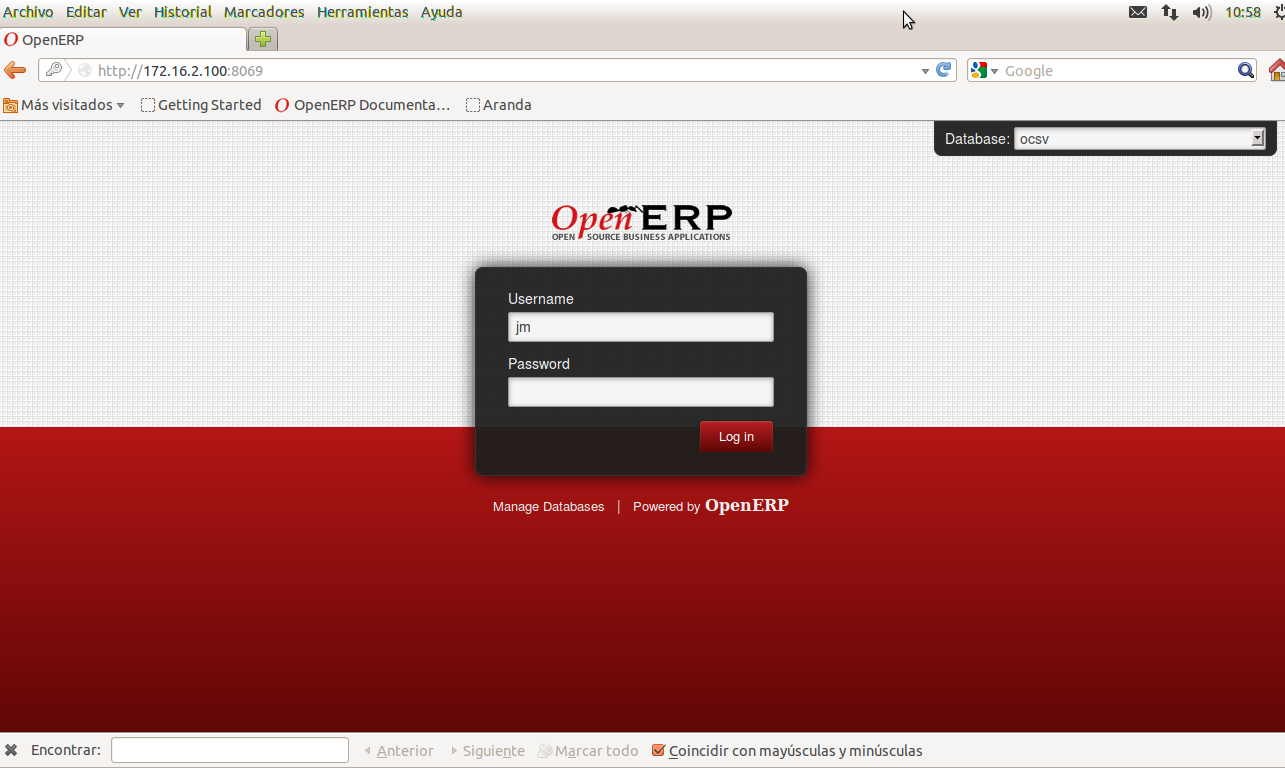
\includegraphics[width=15cm,height=10cm]{./Imagenes/Login.png}
 % Login.png: 1289x610 pixel, 96dpi, 34.10x16.14 cm, bb=0 0 967 457
 \caption{Pantalla de Inicio}
 \label{fig:login}
\end{figure}

\subsection{Entorno de OpenErp}

\begin{itemize}
 \item Si los datos de la cuenta son correctos, la siguiente pantalla muestra el menú principal de la aplicación, tal como lo muestra la figura \ref{fig:menumain}.
 \item Hacer clic en el menú Oficina de Atención al ciudadano $\Rightarrow$ PQR
 \item Aparecerá la lista con las PQR que deben ser tramitadas por el usuario como lo muestra la figura \ref{fig:menulista}
\end{itemize}

\begin{figure}
 \centering
 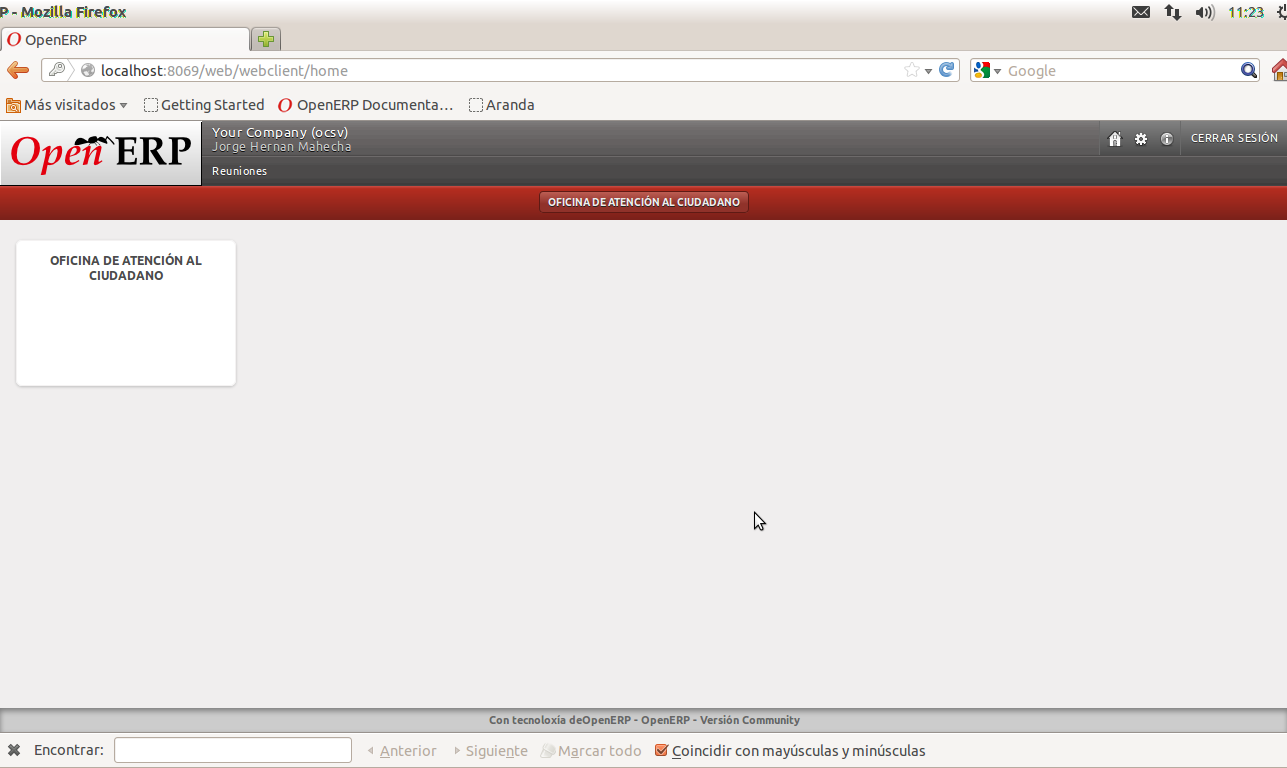
\includegraphics[width=15cm,height=10cm]{./Imagenes/menumain.png}
 % Login.png: 1289x610 pixel, 96dpi, 34.10x16.14 cm, bb=0 0 967 457
 \caption{Menu Principal}
 \label{fig:menumain}
\end{figure}

\begin{figure}
 \centering
 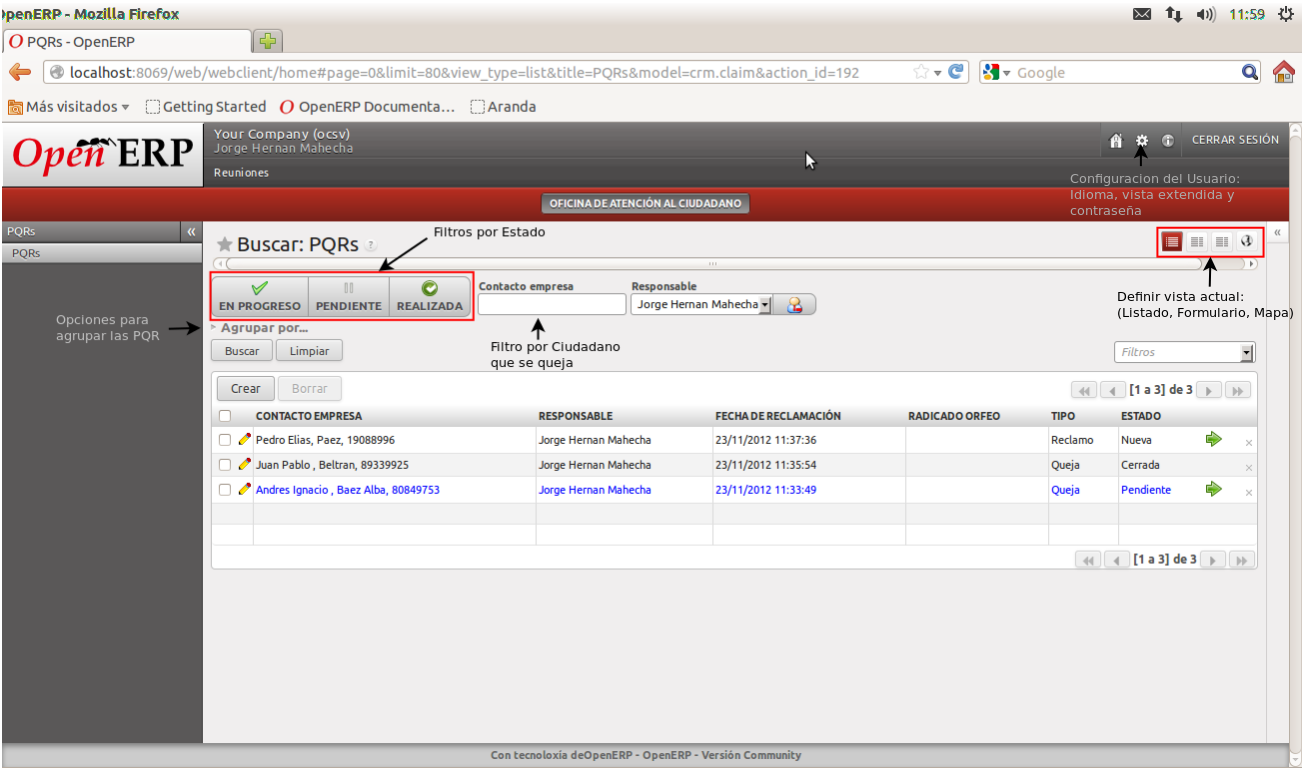
\includegraphics[width=16cm,height=11cm]{./Imagenes/menulista.png}
 % Login.png: 1289x610 pixel, 96dpi, 34.10x16.14 cm, bb=0 0 967 457
 \caption{Lista de PQR}
 \label{fig:menulista}
\end{figure}

\subsection{Funciones Comúnes}


\subsection {Creación de la PQR}

\subsection {Contestando la PQR}

\subsection {Cierre}

\subsection {Agregando Notas}



\subsection{Estados de las PQR}

Las PQR se clasifican por estados, el estado ayuda a conocer como vá el trámite en el que se encuentra la PQR, de esta manera controlar su gestión.
Si se trata de un borrador, la PQR se graba como \textbf{nuevo}, si la PQR ya se encuentra en trámite y la respuesta que se puede dar es casi inmediata
su estado será en \textbf{progreso}, si la PQR no se puede responder rápidamente, debe pasar a un estado \textbf{pendiente}, y si ya se le ha contestado al ciudadano, 
el estado es \textbf{cerrado}, una vez se cierra la PQR ésta no se puede modificar, y su reapertura está reservada para la persona que coordina el 
grupo de usuarios.

\begin{figure}
 \centering
 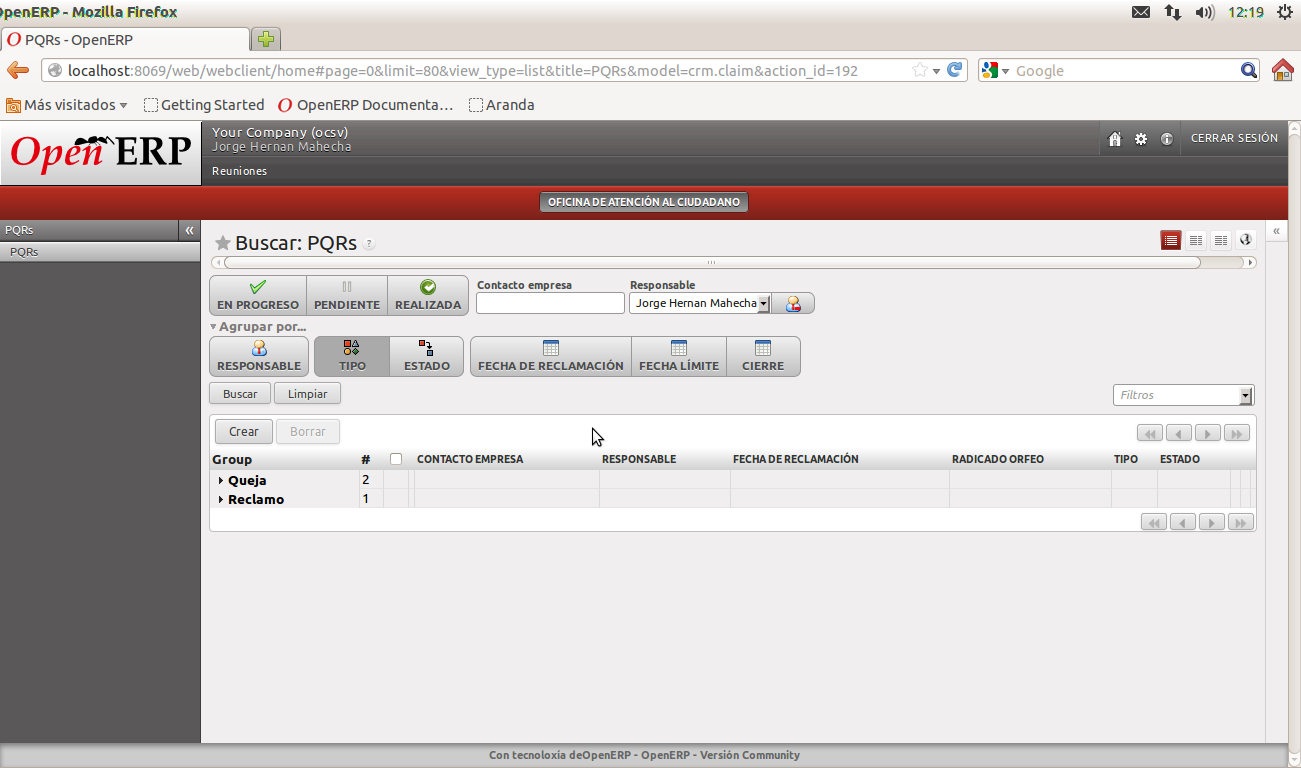
\includegraphics[width=15cm,height=10cm]{./Imagenes/menulistagroup.png}
 % Login.png: 1289x610 pixel, 96dpi, 34.10x16.14 cm, bb=0 0 967 457
 \caption{Agrupando la lista de PQR}
 \label{fig:menulistagroup}
\end{figure}

\begin{figure}
 \centering
 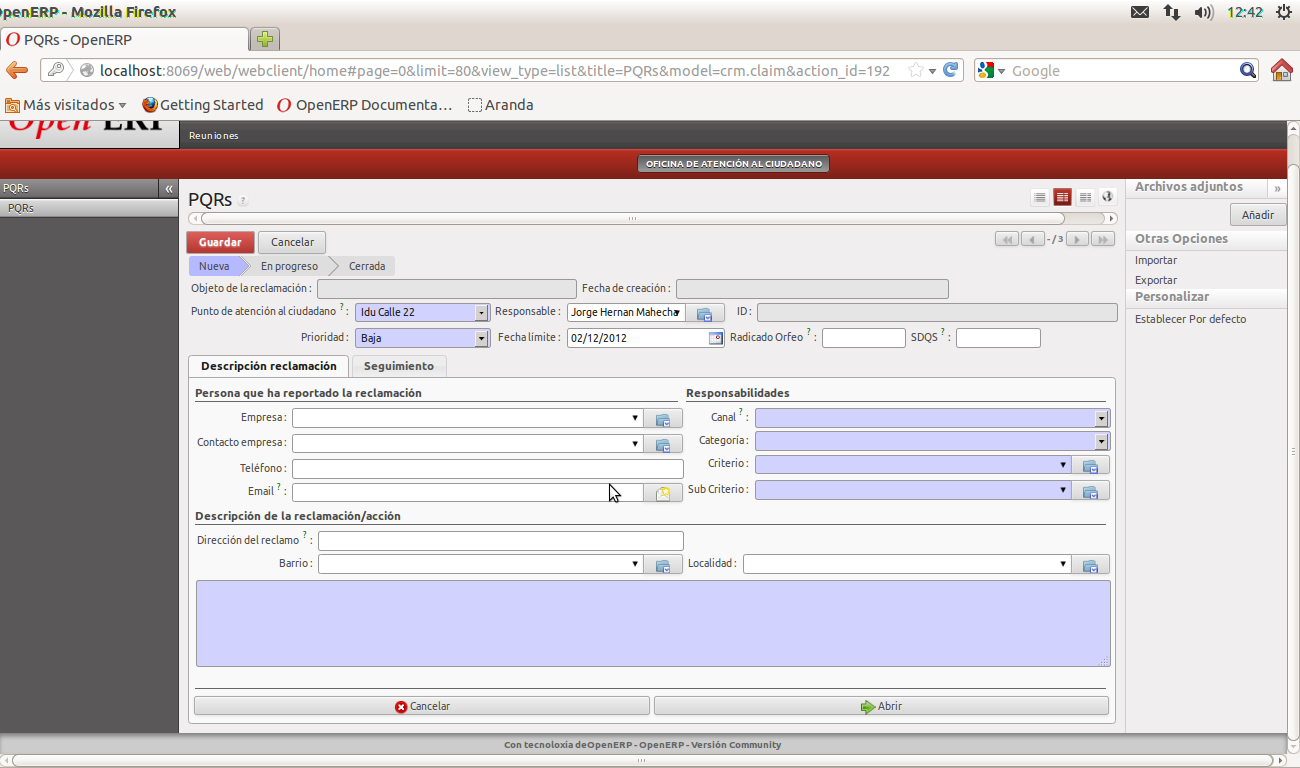
\includegraphics[width=15cm,height=10cm]{./Imagenes/formularioregistro.png}
 % Login.png: 1289x610 pixel, 96dpi, 34.10x16.14 cm, bb=0 0 967 457
 \caption{Registro inicial de la PQR}
 \label{fig:formularioregistro}
\end{figure}

Para facilitar el uso de la herramienta puede agrupar las PQR haciendo clic en el texto \textbf{Agrupar por}, de esta manera puede elegir los siguientes
criterios de agrupación (ver figura \ref{fig:menulistagroup}).
\begin{itemize}
 \item Responsable (Usuario a cargo de la PQR)
 \item Tipo (Petición, Queja, Reclamo, Sugerencia)
 \item Estado (Nuevo, Pendiente, En Progresso, Cerrado)
 \item Fecha de la Reclamación
 \item Fecha Limite
 \item Fecha de Cierre
\end{itemize}


\subsection{Tramitando la PQR}

Para realizar el registro de una PQR se deben seguir los siguientes pasos:

\begin{itemize}
 \item Hacer clic en el botón crear que aparece en la grilla de la Lista, ver figura \ref{fig:menulista} 
 \item Aparecerá el formulario de la figura \ref{fig:formularioregistro}. Los datos inicialmente se  piden son: El usuario que registra 
 la pqr (por defecto), el punto de atención donde se lleva a cabo dicha digitación (IDU, Cade), una prioridad, la fecha límite para tener la respuesta, el número
 de radicación en orfeo si se tiene y el número de radicado de SDQS (Sistema Distrital de Quejas y Soluciones) si se tiene \footnote{En la actualidad 
 se está desarrollando el módulo para llevar a cabo dicho proceso automáticamente}. 
 \item En el campo para anotar los datos de la persona que hace la reclamación, se pueden presentar varios casos: 
 \begin{enumerate}
  \item La queja es anónima: en tal caso el campo donde se relaciona empresa y contacto van vacíos. 
  \item La queja es interpuesta por una empresa: se deben llenar los datos de ésta, y relacionar una persona de contacto. Para ello se deben llenar 
  los datos de la empresa, haciendo clic en el boton anexo al campo 
  \textbf{Empresa} , luego clic en \textbf{Crear}. Aparece una ventana emergente en donde se registran los
  datos básicos de la empresa (ver figura \ref{fig:pantempresa}), como lo es el nombre y el NIT, que se ingresará en el campo (CIF\\NIF). En el siguiente registro
  de persona de contacto se agregan los datos de la persona y se relaciona esta persona a la empresa.
  \item La queja es interpuesta por una persona: Se relacionan los datos de la persona unicamente para ello se llenan los  
  
 \end{enumerate}

\end{itemize}

\begin{figure}
 \centering
 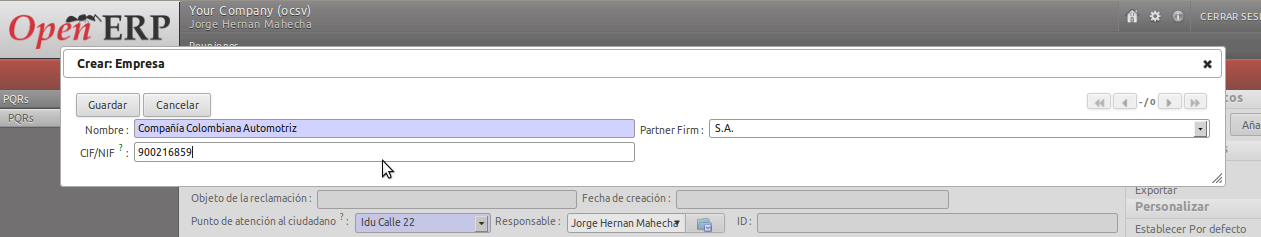
\includegraphics[width=17cm,height=4cm]{./Imagenes/pantempresa.png}
 % Login.png: 1289x610 pixel, 96dpi, 34.10x16.14 cm, bb=0 0 967 457
 \caption{Ventana emergente que solicita datos de la empresa}
 \label{fig:pantempresa}
\end{figure}


\begin{figure}
 \centering
 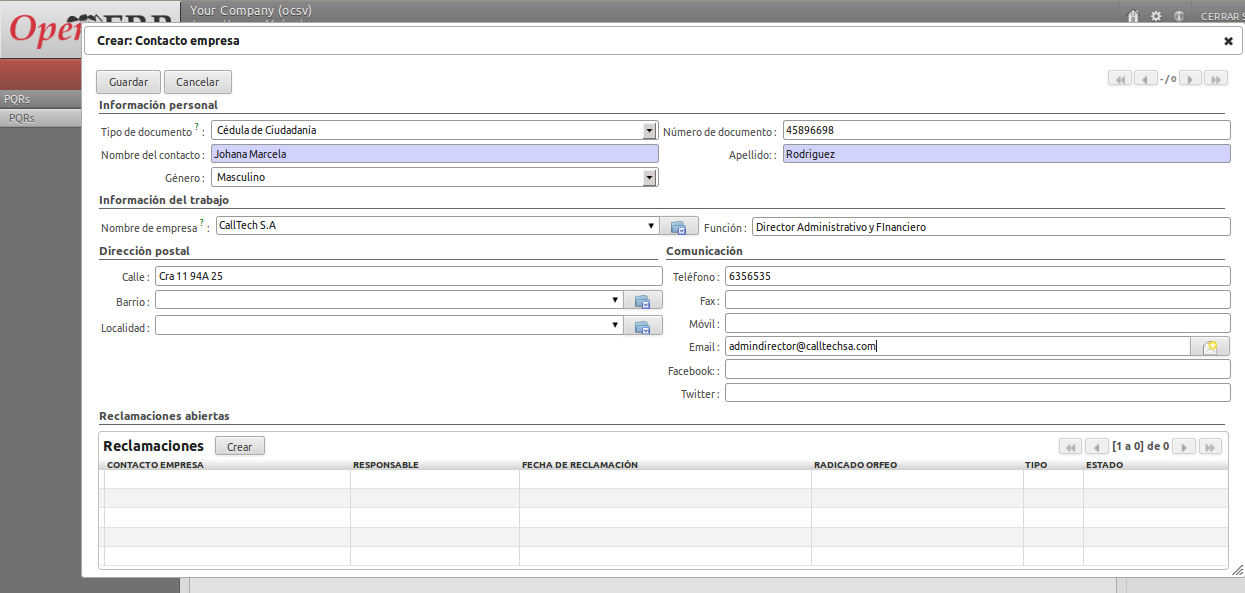
\includegraphics[width=18cm,height=8cm]{./Imagenes/formusuario.png}
 % Login.png: 1289x610 pixel, 96dpi, 34.10x16.14 cm, bb=0 0 967 457
 \caption{Ventana emergente para llenar la información de los usuarios}
 \label{fig:formusuario}
\end{figure}